\documentclass[11pt, oneside]{article}   	% use "amsart" instead of "article" for AMSLaTeX format
\usepackage{geometry}                		% See geometry.pdf to learn the layout options. There are lots.
\geometry{letterpaper}                   		% ... or a4paper or a5paper or ... 
%\geometry{landscape}                		% Activate for for rotated page geometry
%\usepackage[parfill]{parskip}    		% Activate to begin paragraphs with an empty line rather than an indent
\usepackage{graphicx}				% Use pdf, png, jpg, or eps� with pdflatex; use eps in DVI mode
								% TeX will automatically convert eps --> pdf in pdflatex		
\usepackage{amssymb}
\usepackage{amsmath}
\usepackage{parskip}
\usepackage{color}
\usepackage{hyperref}

\title{Video 22:  Morera and L}
%\author{The Author}
%\section{}
%\subsection*{}
\date{}							% Activate to display a given date or no date

\graphicspath{{/Users/telliott_admin/Dropbox/Tex/png/}}
% \begin{center} 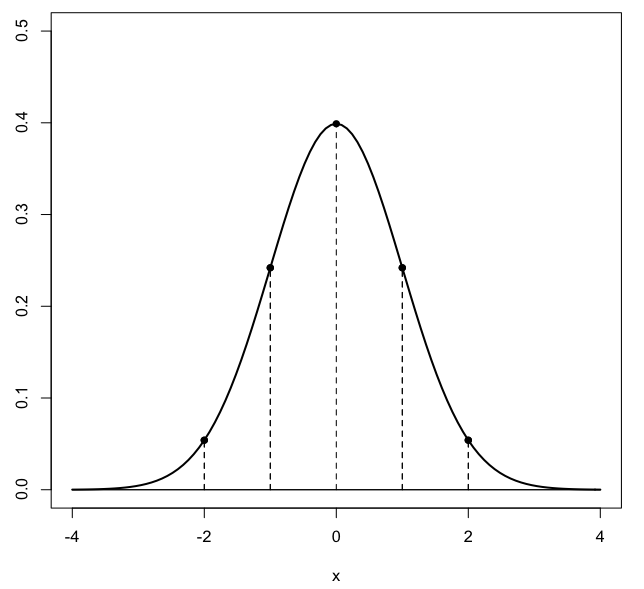
\includegraphics [scale=0.4] {gauss3.png} \end{center}
\begin{document}
\maketitle
\Large
\subsection*{Morera's Theorem}
This is really the converse of Cauchy's Theorem that the line integral of an analytic function $f(z)$ around a closed "nice" curve is equal to zero.

Suppose $f$ is continuous on a domain $D$.  If
\[ \int_{\gamma} f(z) \ dz = 0 \ \ \ \forall \ \text{triangles} \ \gamma \ \text{lying in } D \]
then $f$ is analytic in $D$.
\subsection*{proof}
Let $z_0 \in D$ and $\Omega$ be the disk $\{ z : |z - z_0| < r \}$, with $r > 0$ and small enough so that $\Omega$ is contained in $D$.

Along a closed curve of three line segments joining $z_0 \rightarrow z$, $z \rightarrow z + h$ and then $z+h \rightarrow z_0$, we have that, for $z$ also in $\Omega$:
\[ \int_{z_0}^z f(w) \ dw + \int_{z}^{z+h} f(w) \ dw + \int_{z+h}^{z_0} f(w) \ dw = 0  \]
Moving the third term to the right-hand side, and reversing the path then subtracting the first term, we obtain:
\[  \int_{z}^{z+h} f(w) \ dw =  \int_{z_0}^{z+h} f(w) \ dw -\int_{z_0}^z f(w) \ dw \]
Switch the left- and right-hand sides and using the following new definition:
\[ F(z) = \int_{z_0}^z f(w) \ dw \]
We obtain:
\[ F(z+h) - F(z) = \int_{z}^{z+h} f(w) \ dw  \]

Now, suppose $h$ is a small complex number and we divide both sides by $h$:
\[ \frac{F(z+h) - F(z)}{h} = \int_{z}^{z+h} \frac{ f(w)}{h} \ dw  \]
and subtract $f(z)$
\[ \frac{F(z+h) - F(z)}{h} - f(z) = \int_{z}^{z+h} \frac{ f(w)}{h} \ dw - f(z)  \]
If we consider the line integral of the function $1$ along a path going from $z \rightarrow z + h$ we can write
\[ \int_z^{z+h} \ dw = h \]
so
\[ -f(z) = \frac{-f(z)}{h} \int_z^{z+h} \ dw \]
Both $f(z)$ and $h$ are constants so
\[ -f(z) = - \int_z^{z+h} \frac{f(z)}{h} \ dw \]
Substitute this into what we had above
\[ \frac{F(z+h) - F(z)}{h} - f(z) = \int_{z}^{z+h} \frac{ f(w)}{h} \ dw - \int_z^{z+h} \frac{f(z)}{h} \ dw \]
\[ = \int_{z}^{z+h} \frac{ f(w)-f(z)}{h} \ dw \]

\subsection*{epsilon-delta}
With $\epsilon > 0$ given, we can choose $\delta$ small enough that
\[ | f(w) - f(z) | < \epsilon \]
when
\[ |w-z| < \delta \]
Also choose $|h| < \delta$.  

Then
\[ | \int_z^{z+h} (f(w) - f(z)) \ dw \ | \le  |\epsilon| \int_z^{z+h} dw = \epsilon \ |h| \]
So
\[ | \int_z^{z+h} \frac{f(w) - f(z)}{h} \ dw | \le  \epsilon \]
and
\[ | \frac{F(z+h) - F(z)}{h} - f(z) | =  | \int_z^{z+h} \frac{f(w) - f(z)}{h} \ dw | \le \epsilon \]

So now as $\delta \rightarrow 0$, then $\epsilon \rightarrow 0$ and $h \rightarrow 0$ and so
\[  \lim_{h \rightarrow 0} | \int_{z}^{z+h} \frac{ f(w)-f(z)}{h} \ dw \ | = 0 \]
So we have finally:
\[ \lim_{h \rightarrow 0} \frac{F(z+h) - F(z)}{h} - f(z) = 0 \]
That is:
\[ \lim_{h \rightarrow 0} \frac{F(z+h) - F(z)}{h} =  F'(z) = f(z) \]
So $F(z)$ is differentiable.  And since $F(z)$ is analytic, its derivative $f(z)$ is also analytic.


\end{document}  